% =============================================================================
%  MATE 6026 -- Final Project -- Presentation
%  Compile with: pdflatex main.tex
% =============================================================================
\documentclass[10pt,aspectratio=169]{beamer}

\usetheme{metropolis}
\useinnertheme{default}
\useoutertheme{default}

\usepackage[utf8]{inputenc}
\usepackage{amsmath,amssymb,bm}
\usepackage{graphicx}
\usepackage{booktabs}
\usepackage{algorithm}
\usepackage{algpseudocode}

\newcommand{\R}{\mathbb{R}}
\newcommand{\norm}[1]{\left\|#1\right\|}
\newcommand{\T}{^{\mathsf{T}}}
\newcommand{\grad}{\nabla}

\title{First- and Second-Order Optimization Methods\\ for Neural Network Regression}
\subtitle{Levenberg--Marquardt vs.\ Nonlinear Conjugate Gradient vs.\ Adam}
\author{Author One \and Author Two \and Author Three}
\institute{MATE 6026 --- Numerical Optimization}
\date{\today}

\begin{document}

\maketitle

% ============================================================
\section{Motivation}
% ============================================================

\begin{frame}{The central question}
  \begin{itemize}
    \item Neural networks for regression are almost always trained with
          \alert{Adam} or related first-order adaptive methods.
    \item But MSE-loss regression is, formally, a
          \alert{nonlinear least squares} (NLS) problem.
    \item NLS is Chapter 10 in Nocedal \& Wright: the classical tool is
          \alert{Levenberg--Marquardt (LM)}.
    \vspace{0.5em}
    \item[$\rightarrow$] Does curvature information \emph{actually pay off}
          on a concrete regression problem?
  \end{itemize}
\end{frame}

% ============================================================
\section{Problem formulation}
% ============================================================

\begin{frame}{From regression to nonlinear least squares}
  Given data $\{(x_i, y_i)\}_{i=1}^N$ and network $f(\cdot; \theta)$:
  \begin{equation*}
    r_i(\theta) = y_i - f(x_i; \theta),
    \qquad
    L(\theta) = \tfrac{1}{2}\|r(\theta)\|_2^2.
  \end{equation*}

  Gradient and Gauss--Newton Hessian approximation:
  \begin{equation*}
    \grad L(\theta) = J(\theta)\T r(\theta),
    \qquad
    \grad^2 L(\theta) \approx J(\theta)\T J(\theta).
  \end{equation*}

  \begin{itemize}
    \item $J(\theta) \in \R^{N \times n}$: Jacobian of residuals
    \item Computed analytically via backpropagation
    \item Verified against centered finite differences to $10^{-6}$
  \end{itemize}
\end{frame}

% ============================================================
\section{Three methods}
% ============================================================

\begin{frame}{Levenberg--Marquardt}
  Solve the damped normal equations:
  \begin{equation*}
    (J_k\T J_k + \lambda_k I)\, p_k = -J_k\T r_k,
    \qquad \theta_{k+1} = \theta_k + p_k.
  \end{equation*}
  Accept/reject based on the gain ratio; increase $\lambda$ on reject
  (toward steepest descent), decrease on accept (toward Gauss--Newton).
  \vspace{1em}

  Uses: full residual Jacobian + exact curvature (Gauss--Newton).
\end{frame}

\begin{frame}{Nonlinear Conjugate Gradient}
  Polak--Ribi\`ere${}^+$ direction:
  \begin{align*}
    \beta_{k+1}^{\mathrm{PR+}}
    &= \max\!\left\{\frac{g_{k+1}\T(g_{k+1}-g_k)}{g_k\T g_k},\; 0\right\} \\
    p_{k+1} &= -g_{k+1} + \beta_{k+1}^{\mathrm{PR+}} p_k.
  \end{align*}
  Step length from strong Wolfe line search; restart every $n$ iters.
  \vspace{1em}

  Uses: gradients only (no curvature).
\end{frame}

\begin{frame}{Adam}
  Mini-batch first- and second-moment estimates:
  \begin{align*}
    m_k &= \beta_1 m_{k-1} + (1-\beta_1) \tilde{g}_k \\
    v_k &= \beta_2 v_{k-1} + (1-\beta_2) \tilde{g}_k \odot \tilde{g}_k \\
    \theta_{k+1} &= \theta_k - \alpha\, \hat{m}_k \oslash (\sqrt{\hat{v}_k} + \epsilon)
  \end{align*}

  Uses: stochastic gradients + \emph{diagonal} second-moment estimate.
\end{frame}

% ============================================================
\section{Experimental setup}
% ============================================================

\begin{frame}{Setup}
  \begin{itemize}
    \item \textbf{Dataset:} UCI Concrete Compressive Strength (1030 samples, 8 features)
    \item \textbf{Architecture:} $8 \to 16 \to 16 \to 1$ with tanh hidden,
          linear output ($n=433$ parameters)
    \item \textbf{Split:} 70/15/15 stratified by target quantile
    \item \textbf{Seeds:} five, same $\theta_0$ per seed across all three methods
    \item \textbf{Stopping:} $\norm{\grad L}_\infty < 10^{-5}$ (LM, NCG); Adam with
          validation early stopping (patience 50)
    \item \textbf{Adam LR:} tuned on seed 0 over
          $\{10^{-4}, 3\!\cdot\!10^{-4}, 10^{-3}, 3\!\cdot\!10^{-3}, 10^{-2}\}$
  \end{itemize}
\end{frame}

% ============================================================
\section{Results}
% ============================================================

\begin{frame}{Convergence per iteration}
  \centering
  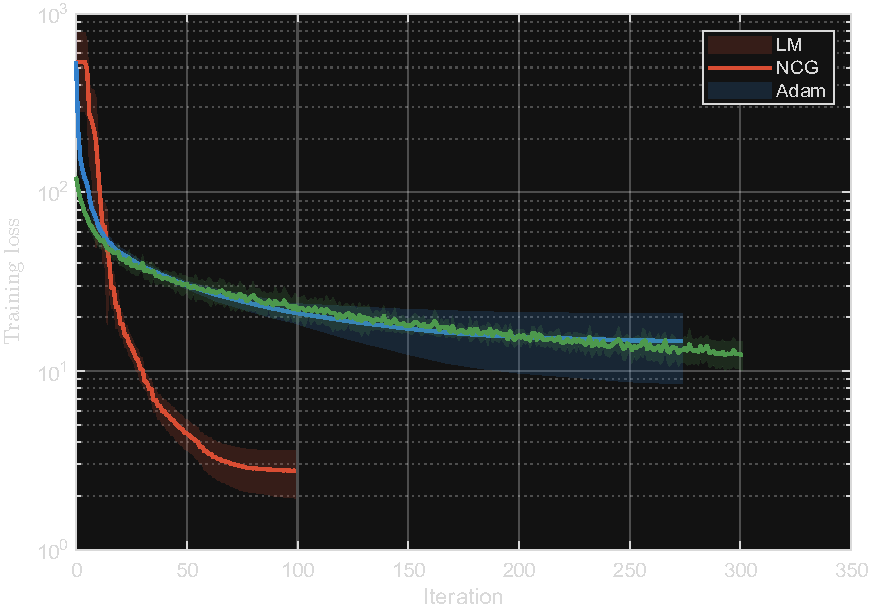
\includegraphics[width=0.75\linewidth]{../report/figures/loss_vs_iter.pdf}

  \small
  LM converges in far fewer iterations; NCG and Adam more gradually.
\end{frame}

\begin{frame}{Wall-clock efficiency}
  \centering
  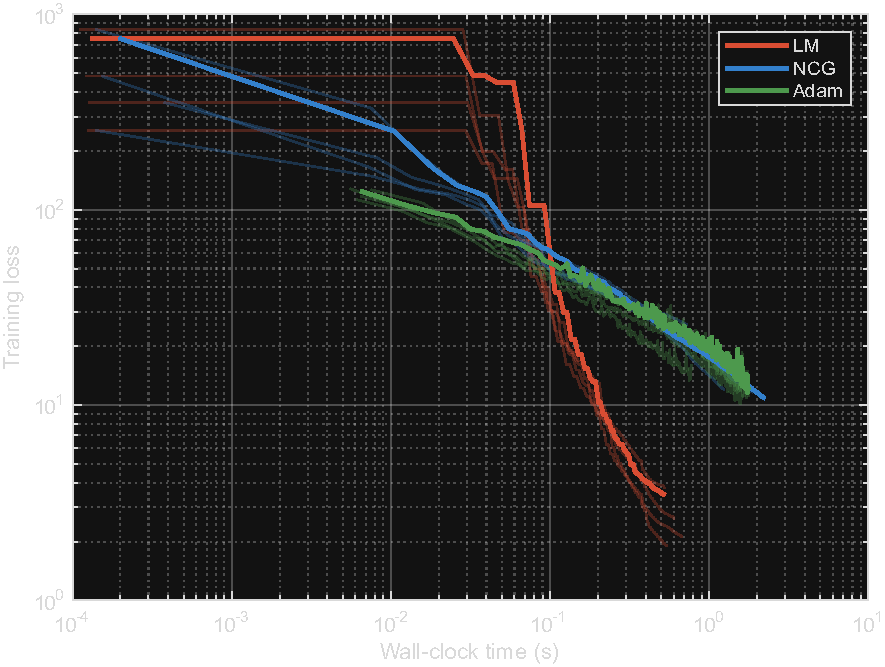
\includegraphics[width=0.75\linewidth]{../report/figures/loss_vs_time.pdf}

  \small
  Per-iteration cost differs: LM solves a 433$\times$433 system;
  Adam is mostly mini-batch gradient evaluations.
\end{frame}

\begin{frame}{Generalization: test RMSE}
  \centering
  \begin{tabular}{@{}lrrrr@{}}
    \toprule
    Method & Train RMSE & Val RMSE & Test RMSE & Time (s) \\
    \midrule
    LM   & \texttt{[X $\pm$ X]} & \texttt{[X $\pm$ X]} & \texttt{[X $\pm$ X]} & \texttt{[X $\pm$ X]} \\
    NCG  & \texttt{[X $\pm$ X]} & \texttt{[X $\pm$ X]} & \texttt{[X $\pm$ X]} & \texttt{[X $\pm$ X]} \\
    Adam & \texttt{[X $\pm$ X]} & \texttt{[X $\pm$ X]} & \texttt{[X $\pm$ X]} & \texttt{[X $\pm$ X]} \\
    \bottomrule
  \end{tabular}
  \vspace{1em}

  \small
  (Values in MPa, mean $\pm$ std over five seeds.)
\end{frame}

\begin{frame}{Predicted vs.\ actual (test set)}
  \centering
  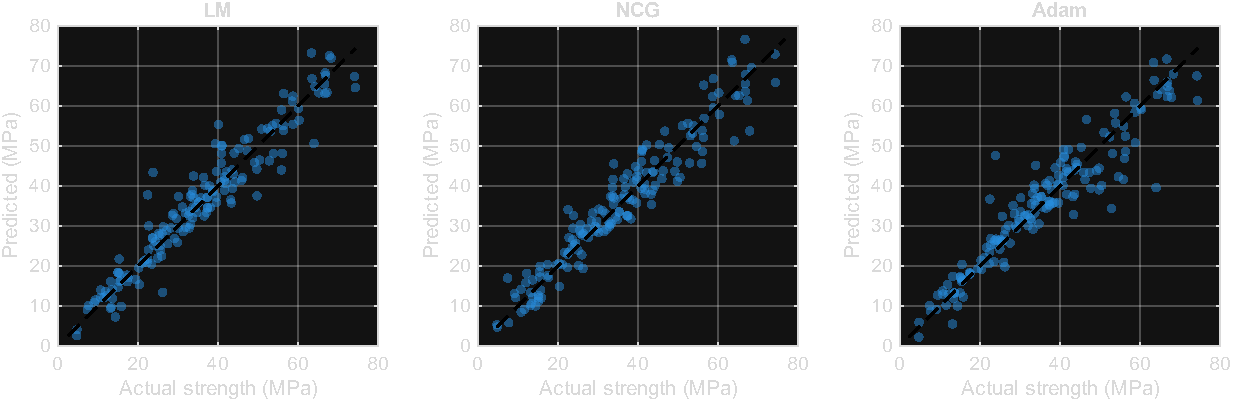
\includegraphics[width=0.95\linewidth]{../report/figures/pred_vs_actual.pdf}
\end{frame}

\begin{frame}{LM diagnostic: damping trajectory}
  \centering
  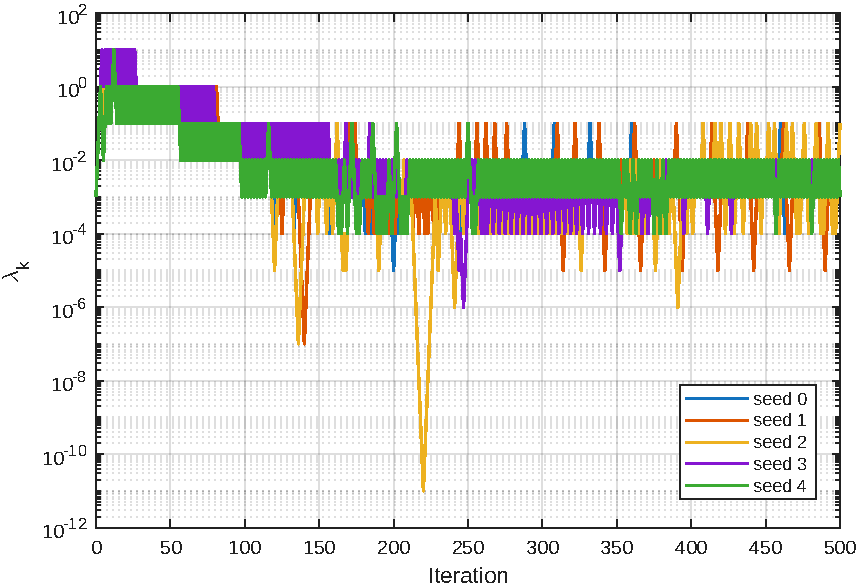
\includegraphics[width=0.7\linewidth]{../report/figures/lm_lambda.pdf}

  \small
  $\lambda_k$ starts near steepest-descent territory and decays toward
  Gauss--Newton behavior as the iterates approach a minimizer.
\end{frame}

% ============================================================
\section{Conclusions}
% ============================================================

\begin{frame}{Does curvature information pay off?}
  \begin{itemize}
    \item \textbf{Per iteration:} LM wins clearly --- exploiting $J\T J$
          drives the loss down fast.
    \item \textbf{Per second:} \texttt{[fill in after experiments]}.
    \item \textbf{Generalization:} \texttt{[fill in]} --- test RMSE across
          the three methods is comparable, suggesting that at this problem
          scale the bottleneck is data/representation, not the optimizer.
  \end{itemize}
  \vspace{1em}
  \alert{Takeaway:} for small-to-medium NLS problems, LM remains
  competitive with Adam in accuracy and often wins in iterations;
  wall-clock depends on the linear-solve cost vs.\ Adam's mini-batch noise.
\end{frame}

\begin{frame}{Limitations and future work}
  \begin{itemize}
    \item Single dataset; no architecture sweep.
    \item LM/NCG are full-batch; Adam is mini-batch --- a genuine
          asymmetry in the comparison.
    \item LM's $O(n^3)$ linear solve bites for larger networks; scaling
          up would shift the wall-clock picture.
    \item Future: subsampled Gauss--Newton (stochastic LM), L-BFGS as a
          middle ground.
  \end{itemize}
\end{frame}

\begin{frame}[standout]
  Questions?
\end{frame}

\end{document}
